%!TEX program = xelatex
\documentclass[dvipsnames, svgnames,a4paper,11pt]{article}
% ----------------------------------------------------
%   中山大学物理与天文学院本科实验报告模板
%   作者:Huanyu Shi,2019级
%   知乎:https://www.zhihu.com/people/za-ran-zhu-fu-liu-xing
%   Github:https://github.com/huanyushi/SYSU-SPA-Labreport-Template
%   Last update : 2023.4.10
% ----------------------------------------------------

% ----------------------------------------------------- 
%	加边框的命令
%	参考:https://tex.stackexchange.com/questions/531559/how-to-add-the-page-border-for-first-two-pages-in-latex
\usepackage{tikz}
\usetikzlibrary{calc}
\usepackage{eso-pic}
\AddToShipoutPictureBG{%
\begin{tikzpicture}[overlay,remember picture]
\draw[line width=0.6pt] % 边框粗细
    ($ (current page.north west) + (0.6cm,-0.6cm) $)
    rectangle
    ($ (current page.south east) + (-0.6cm,0.6cm) $); % 边框位置
\end{tikzpicture}}


\usepackage{xcolor}
\definecolor{c1}{HTML}{2752C9} % 目录颜色
\definecolor{c2}{RGB}{190,20,83} % 引用颜色

\usepackage{ctex}
\usepackage[top=28mm,bottom=28mm,left=15mm,right=15mm]{geometry}
\usepackage{hyperref} 
\hypersetup{
	colorlinks,
	linktoc = section, % 超链接位置,选项有section, page, all
	linkcolor = c1, % linkcolor 目录颜色
	citecolor = c1  % citecolor 引用颜色
}
\usepackage{amsmath,enumerate,multirow,float}
\usepackage{tabularx}
\usepackage{tabu}
\usepackage{subfig}
\usepackage{fancyhdr}
\usepackage{graphicx}
\usepackage{wrapfig}  
\usepackage{physics}
\usepackage{appendix}
\usepackage{amsfonts}

%
\usepackage{tcolorbox}
\tcbuselibrary{skins,breakable}
\newtcolorbox{tbox}[2][]{
    colframe=black!70!,
    breakable,
    enhanced,
	boxrule =0.5pt,
    title = {#2},
    fonttitle = \large\kaishu\bfseries,
	drop fuzzy shadow,
    #1
}
\newtcolorbox[auto counter,number within=section]{question}[1][]{
  top=2pt,bottom=2pt,arc=1mm,
  boxrule=0.5pt,
%   frame hidden,
  breakable,
  enhanced, %跨页后不会显示下边框
  coltitle=c1!80!gray,
  colframe=c1,
  colback=c1!3!white,
  drop fuzzy shadow,
  title={思考题~\thetcbcounter:\quad},
  fonttitle=\bfseries,
  attach title to upper,
  #1
}

% ---------------------------------------------------------------------
%	利用cleveref改变引用格式,\cref是引用命令
\usepackage{cleveref}
\crefformat{figure}{#2{\textcolor{c2}{图 #1}}#3} % 图片的引用格式
\crefformat{equation}{#2{(\textcolor{c2}{#1})}#3} % 公式的引用格式
\crefformat{table}{#2{\textcolor{c2}{表 #1}}#3} % 表格的引用格式


% ---------------------------------------------------------------------
%	页眉页脚设置
\fancypagestyle{plain}{\pagestyle{fancy}}
\pagestyle{fancy}
\lhead{\kaishu 中山大学物理与天文学院基础物理实验\uppercase\expandafter{\romannumeral2}} % 左边页眉,学院 + 课程
\rhead{\kaishu  \quad 光学相差实验Ⅰ} % 右边页眉,实验报告标题
\cfoot{\thepage} % 页脚,中间添加页码


% ---------------------------------------------------------------------
%	对目录、章节标题的设置
\renewcommand{\contentsname}{\centerline{\huge 目录}}
\usepackage{titlesec}
\usepackage{titletoc}
% \titleformat{章节}[形状]{格式}{标题序号}{序号与标题间距}{标题前命令}[标题后命令]
\titleformat{\section}{\centering\LARGE\songti}{}{1em}{}

% ---------------------------------------------------------------------
%   listing代码环境设置
\usepackage{listings}
\lstloadlanguages{python}
\lstdefinestyle{pythonstyle}{
backgroundcolor=\color{gray!5},
language=python,
frameround=tftt,
frame=shadowbox, 
keepspaces=true,
breaklines,
columns=spaceflexible,                   
basicstyle=\ttfamily\small, % 基本文本设置,字体为teletype,大小为scriptsize
keywordstyle=[1]\color{c1}\bfseries, 
keywordstyle=[2]\color{Red!70!black},   
stringstyle=\color{Purple},       
showstringspaces=false,
commentstyle=\ttfamily\scriptsize\color{green!40!black},%注释文本设置,字体为sf,大小为smaller
tabsize=2,
morekeywords={as},
morekeywords=[2]{np, plt, sp},
numbers=left, % 代码行数
numberstyle=\it\tiny\color{gray}, % 代码行数的数字字体设置
stepnumber=1,
rulesepcolor=\color{gray!30!white}
}




% ---------------------------------------------------------------------
%	其他设置
\def\degree{${}^{\circ}$} % 角度
\graphicspath{{./images/}} % 插入图片的相对路径
\allowdisplaybreaks[4]  %允许公式跨页 % 导入模板的相关设置
\usepackage{lipsum}
\usepackage{enumitem}
\usepackage{tabularray}  %绘制表格时可以更加方便添加框线
\usepackage{xcolor} %添加更多文本颜色

\setlist[enumerate]{label=\textup{(\arabic*)}}



%---------------------------------------------------------------------
%	正文
%---------------------------------------------------------------------

\begin{document}


% \begin{table}
% 	\renewcommand\arraystretch{1.7}
% 	\begin{tabularx}{\textwidth}{
% 		|X|X|X
% 		|X|X|X|}
% 	\hline
% 	\multicolumn{2}{|c|}{预习报告}&\multicolumn{2}{|c|}{实验记录与分析}&\multicolumn{2}{|c|}{总成绩}\\
% 	\hline
% 	\LARGE30 & & \LARGE50 & & \LARGE80 & \\
% 	\hline
% 	\end{tabularx}
% \end{table}

\begin{table}
	\renewcommand\arraystretch{1.7}
	\begin{tabularx}{\textwidth}{
		|>{\centering}X|>{\centering}X|>{\centering}X
		|>{\centering}X|>{\centering}X|>{\centering\arraybackslash}X|}
	\hline
	\multicolumn{2}{|c|}{预习报告}&\multicolumn{2}{c|}{实验记录与分析}&\multicolumn{2}{c|}{总成绩}\\
	\hline
	\LARGE30 & & \LARGE50 & & \LARGE80 & \\
	\hline
	\end{tabularx}
\end{table}


\begin{table}
	\renewcommand\arraystretch{1.7}
	\begin{tabularx}{\textwidth}{|X|X|X|X|}
	\hline
	年级、专业:& 物理学 &组号:& 实验班2\\
	\hline
	姓名:& 戴鹏辉  & 学号: & 2344016 \\
	\hline
	日期:& 2024/03/17 & 教师签名:& \\
	\hline
	\end{tabularx}
\end{table}

\begin{center}
	\LARGE 全息照相实验
\end{center}

\textbf{【实验报告注意事项】}
\begin{enumerate}[label=\arabic*., leftmargin=*]
	\item 实验报告由两部分组成:
		\begin{enumerate}[label=\arabic*), leftmargin=*]
			\item 预习报告:课前认真研读\underline{\textbf{实验讲义}},弄清实验原理;实验所需的仪器设备、用具及其使用、完成课前预习思考题;了解实验需要测量的物理量,并根据要求提前准备实验记录表格(可以参考实验报告模板,可以打印)。\textcolor{red}{\textbf{(30分)}}
			\item 实验记录与分析:认真、客观记录实验条件、实验过程中的现象以及数据。实验记录请用珠笔或者钢笔书写并签名(\textcolor{red}{\textbf{用铅笔记录的被认为无效}})。\textcolor{red}{\textbf{保持原始记录,包括写错删除部分,如因误记需要修改记录,必须按规范修改。}}(不得手记的值输入到电脑打印);离开前请实验教师检查记录并签名。\textcolor{red}{\textbf{(50分)}}
		\end{enumerate}
	
	\item \textcolor{red}{\textbf{本实验报告可提前打印出来,当场记录分析完成交给带实验的老师,课后无需再提交。若当场完成不了,则请课后完成,再扫描并通过seelight提交。}}
	
	\textcolor{red}{\textbf{注意:本文档已留出填写空间,若填写空间不够的话请提前规划留白,做到报告的美观}}
	\item 注意事项:
		\begin{enumerate}[label=\arabic*), leftmargin=*]
			\item 实验中\textcolor{red}{\textbf{避免激光器伤到眼睛}}
			\item 避免用手直接接触镜片的光学面
			\item 安装镜片时需在光学平台上尽量靠近台面的高度操作,以免失手跌落摔碎镜片
			\item 实验平台配件所用固定螺钉需拧紧,以免镜架晃动;但不可过紧,以免损坏
			\item 实验前需按仪器清单检查光学元件是否齐全,\textcolor{red}{\textbf{实验结束后按照顺序放回元件盒}}
			
		\end{enumerate}
\end{enumerate}


\clearpage
\tableofcontents
\clearpage

\setcounter{section}{0}
\section{全息照相实验 \quad\heiti 预习报告}
	
\subsection{实验目的}
	\begin{enumerate}
		\item 学习全息照相的基本原理和方法;
		\item 了解全息照相的主要特点;
		\item 学习全息照片的制作方法和技术;
		\item 学习观察全息照片的方法。
		
		
	\end{enumerate}

\subsection{仪器用具}
\begin{table}[htbp]
	\centering
	\renewcommand\arraystretch{1.6}
	% \setlength{\tabcolsep}{10mm}
	\begin{tabular}{p{0.05\textwidth}|p{0.20\textwidth}|p{0.05\textwidth}|p{0.5\textwidth}}
	\hline
	编号& 仪器用具名称 & 数量 &  主要参数(型号,测量范围,测量精度等) \\
	\hline
	1  & 防震光学平台 & 1  & ~  \\
	2  & 氦氖激光器  & 1  & ~  \\
	3  & 扩束透镜   & 1  & ~  \\
	4  & 分束器    & 1  & ~  \\
	5  & 反射镜    & 3  & ~  \\
	6  & 全息干版   & 1  & ~  \\
	7  & 显影液    & 1  & ~  \\
	8  & 定影液    & 1  & ~  \\
	9  & 暗房设备   & 1  & ~  \\
	\hline
\end{tabular}
\end{table}

\subsection{原理概述}
	
	全息照相是一种不用透镜而能记录和再现物体的三维(立体)图象的照相方法,能够把来自物体的光波波前的振幅和相位信息完整记录下来, 并能够完整的再现出物体的三维图像。在实验应力分析、图象识别和无损检验、照相领域等具有广泛应用。
	
	\begin{enumerate}
		\item \textbf{全息照相的特点}:
		
			全息照相与普通照相原理有本质差别。普通照相利用透镜将物体成像在平面上,记录各点的光强或振幅分布,但仅为二维像。全息照相则利用光的干涉、衍射等规律,记录物光波的振幅与位相的全部信息,得到细密干涉条纹,称为全息图。全息照片具有以下特点:
			\begin{itemize}
				\item 重建物光波与原物光波具有相同的深度和视差,观察位置变化可看到景物被遮拦的物体,需要重新调焦;
				
				\item 每小块全息照片都可再现整个图像,因每点包含整个图像信息,但随小块减小,分辨率逐渐变差;
				
				\item 可用接触法复制,无正负片之分,且再现影像的反差接近原物体;
				
				\item 绕不同轴线转动全息照片产生不同效果;
				
				\item 连续曝光可重叠几个影像,每个影像单独显现。
			\end{itemize}
		\item \textbf{物理原理}
			
			全息照相是一种使用相干光源进行的两步光学成像过程,在第一步中,参考光和物光在记录介质上形成复杂的干涉图样,称为全息图;在第二步中,通过适当的照明,从全息图中再现出物体通常的图像。
			
			全息照相的基本理论实质上是一种较为广义的双光束干涉场的计算。使用激光器发出的相干光经过分束器分为两束,一束照明物体成为景物光,另一束作为参考光。这两束光以一定的夹角入射到记录介质上相互干涉,形成全息图。由于记录介质只能记录振幅,可见物波的位相记录也是利用干涉的原理转换成相应的振幅关系加以记录的。
			
				\begin{enumerate}[label=\roman*.]
					\item 全息照相记录的信号
						设$O$和$R$分别为物光和参考光
						\[
						\left\{
						\begin{aligned}
							& O(r,t)=A_0(r)e^{i(\phi_0-\omega t)}\\
							& R(r,t)=A_R(r)e^{i(\phi_R-\omega t)}
						\end{aligned}
						\right.
						\]
						则光强度为:
						\[
						I(r,t)=(O+R)^2=\left| O \right|^2+\left| R \right|^2+2\left| O \right|\left| R \right|\cos(\phi_0-\phi_R)
						\]
						由于做全息照相时,总是尽量让参考光和物光各自在记录介质上的照度均匀,所以这里主要关注相干项。\\
						干涉项产生的是明暗以$(\phi_0-\phi_R)$为变量按余弦规律变化的干涉条纹并被记录介质记录下来。由于这些干涉条纹在记录介质上各点的强度决定于物光波(以及参考光波)在各点的振幅和相位,因此记录介质上就保留了物光波的振幅和相位信息。

					\item 波前重现
					设全息底片工作于线性区,则经显影、定影等处理后,其振幅透过率与曝光强度成正比:
					\[
					\tau(x,y)=\tau_0+\beta I(x,y)=\tau_0+\beta\left[\left|O\right|^2+\left|R\right|^2+R^*\left|O\right|+R\left|O\right|^*\right]\quad (\beta<0)
					\]

					当用原参考光重现时,其透射光场为:
					\[
					A_{rec}(r,t)=R(r,t)\tau(r)=R\left[\tau_0+\beta\left(\left|O\right|^2+\left|R\right|^2\right)\right]+\beta RR^*O+\beta R^2O	
					\]
					当用共轭参考光重现时,其透射光场为:
					\[
					A_{rec}(r,t)=R^*(r,t)\tau(r)=R^*\left[\tau_0+\beta\left(\left|O\right|^2+\left|R\right|^2\right)\right]+\beta (R^*)^2O+\beta \left|R\right|^2O^*	
					\]
					说明:前面两个公式表现出曝光时的入场光场和显影后的透射光场之间的高度非线性关系,似乎线性系统对全息照相理论不起作用。但是从物光场$O(x,y)$到透射光场分量$E_\epsilon=\beta \left|R\right|^2O$或$E'_\epsilon=\beta \left|R\right|^2O^*$的变换确实完全线性的。

					\begin{figure}[htbp]
						\centering
						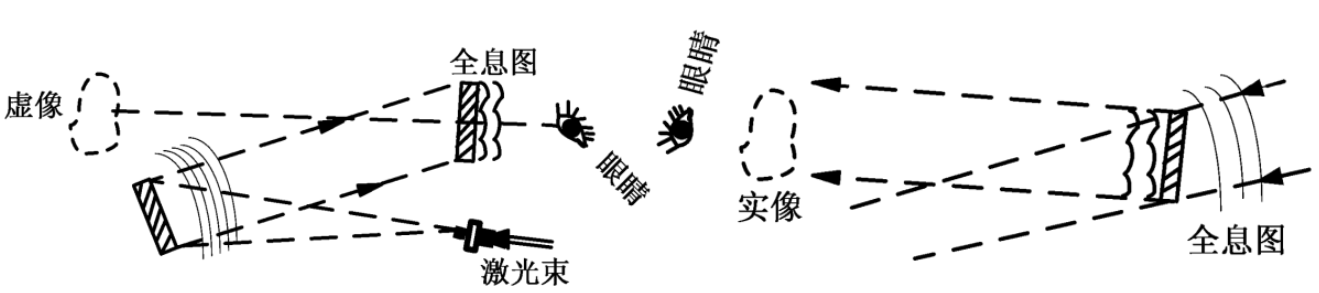
\includegraphics[width=0.85\textwidth]{graph1.png}
						\caption{全息图的波前重建}
						\label{fig:graph1}
					\end{figure}

				\end{enumerate}
			
			
			
		\item 实验条件
			
			\textbf{对稳定性的要求}:
				\begin{enumerate}[label=\roman*.]
					\item 干涉条纹非常细密,极小的扰动会导致干涉模糊,甚至无法记录下来。
					\item 景物在曝光时间内移动 $\lambda/8$ 就足以使干涉条纹模糊不清,因此曝光期间,元件之间的相对位移应小于条纹间距的几分之一。
					\item 空气、声波和温度的变化会引起元件的震动或空气密度不均匀,需避免大声喧哗、敲门、吹风等,更不能碰到防震台。
					\item 缩短曝光时间有利于减少外界震动的影响,但受光源强度和底片灵敏度限制。
				\end{enumerate}
	 
			\textbf{对光源相干性的要求}:
				\begin{enumerate}[label=\roman*.]
					\item 参考光束与物光束必须是相干的,使用 $He-Ne$ 激光器等相干光源。
					\item 激光器的谱线有一定宽度,考虑多普勒展宽等因素,相干长度应足够长。
					\item 参考光路与物光路的光程应接近相等,被摄景物的景深应在相干长度之内。
					\item 选用单横模(TEM00)的激光器,景物的大小应在空间相干的范围内。
				\end{enumerate}

			 这些要求保证了全息照相的稳定性和记录质量。

	\end{enumerate}

\subsection{实验前思考题}
	\begin{question}
		实验中应该注意哪些影响因素才能够保证成功观察到全息再现图像?
	\end{question}
		
		\begin{enumerate}[label=\roman*.]
			\item \textbf{稳定性要求}:
			全息照片制备过程中,曝光期间元件之间的相对位移应小于干涉条纹间距的几分之一,以避免干涉条纹模糊不清。
			避免外界因素(如空气、声波、温度变化)对元件的震动或空气密度不均匀,需避免大声喧哗、敲门、吹风等,更不能碰到防震台。
			
			\item \textbf{光源相干性要求}:	
			参考光束与物光束必须是相干的,使用 He-Ne 激光器等相干光源。
			参考光路与物光路的光程应接近相等,被摄景物的景深应在相干长度之内。

			\item \textbf{曝光时间和光源强度}:
			缩短曝光时间有利于减少外界震动的影响,但受光源强度和底片灵敏度限制。
			光源强度应足够,以保证充分的曝光。

			\item \textbf{干涉条纹清晰度}:
			景物在曝光时间内移动 λ/8 就足以使干涉条纹模糊不清,因此曝光期间,应保持元件稳定不动。
			
			\item \textbf{实验环境}:
			实验室环境应保持安静,避免震动和空气流动对实验造成影响。
			应该在光学平台上进行实验,以减少振动和移动。

			\item \textbf{底片和显影过程}:
			底片的选择和显影过程也会影响全息再现图像的质量,需要按照标准操作程序进行处理。
			
		\end{enumerate}
	
		综上所述,保证实验环境稳定、光源相干性良好、曝光时间合适以及注意底片和显影过程等因素都是保证成功观察到全息再现图像的关键。
		
		
		
		

	\begin{question}
		物光和参考光的光程差应保持在什么范围?为什么?
	\end{question}
		
	% 物光和参考光的光程差应该尽可能小,通常应保持在相干长度的范围内。光程差过大会导致相干性减弱,干涉条纹变得模糊或消失,从而影响全息图的质量。相干长度越小,两束光的光程差就越难以控制,因此需要尽可能小地保持物光和参考光的光程差,以确保干涉条纹清晰可见,从而获得高质量的全息再现图像。

	在全息照相中,物光和参考光的光程差对干涉条纹的质量有着直接影响。当两束光波在全息底片上相遇并叠加时,如果它们的光程相等或非常接近,就能够会产生稳定的干涉图案。这是因为光波的相位关系保持一致,从而形成清晰的干涉条纹。

	干涉条纹的清晰度对全息图的质量至关重要。如果光程差过大,超过了激光的相干长度,两束光波的相位就会失去同步,导致干涉条纹模糊或完全消失。

	为了确保高质量的干涉条纹,物光和参考光的光程差应控制在激光的相干长度范围内,这样可以保证两束光在全息底片上产生高对比度和清晰度的干涉条纹,从而生成高质量的全息图。

\clearpage
\begin{table}
	\renewcommand\arraystretch{1.7}
	\centering
	\begin{tabularx}{\textwidth}{|X|X|X|X|}
	\hline
	专业:& 物理学 &年级:& 2022级 \\
	\hline
	姓名:& 戴鹏辉 & 学号:& 22344016 \\
	\hline
	室温:&  & 实验地点: &  \\
	\hline
	学生签名:& & 评分: &\\
	\hline
	日期:&  & 教师签名:&\\
	\hline
	\end{tabularx}
\end{table}

\section{全息照相实验 \quad\heiti 实验记录}
\subsection{实验内容、步骤、结果及讨论}\textcolor{ForestGreen}{(按照实验顺序依次}\textcolor{red}{简要记录}\textcolor{ForestGreen}{实验内容及步骤,)(空间不够,可自行加页)}\\
\textcolor{red}{
(注意: \\
除了记录实验内容、步骤、参数外,还应记录:\\
按比例绘制操作中实际摆放的实验光路(各元件间距离可通过直尺测量)\\
记录光路中物光和参考光的光程差\\
记录物光和参考光光强比\\
记录是否可观察到再现图像\\
)
}


		

%\subsection{实验数据记录}



%\subsection{原始数据记录}

\clearpage

\newpage

\null

\newpage

\null






\newpage

\subsection{实验过程中遇到的问题记录}

	\begin{enumerate}
		\item 
		\item 
		\item 
	\end{enumerate}
\null




% \begin{table}
% 	\renewcommand\arraystretch{1.7}
% 	\begin{tabularx}{\textwidth}{|X|X|X|X|}
% 	\hline

% 	专业:& 物理学 &年级:& 2022级\\
% 	\hline
% 	姓名: & 戴鹏辉 & 学号:& 22344016\\
% 	\hline
%     日期:& 2024/xx/xx & 评分: &\\
% 	\hline
% 	\end{tabularx}
% \end{table}

% \section{全息照相实验 \quad\heiti 分析与讨论}

% \subsection{实验数据分析}

% 	\subsubsection{实验一 测量光栅常数}
	
		
% 	\subsubsection{实验二 测定未知光波波长及角色散率D}
			

			
% \subsection{实验后思考题}



% \begin{question}
% 	检索文献,列举三种测量光波波长的方法,给出参考文献列表。%\lipsum[20]
% \end{question}
	

	



\end{document}
